
\documentclass[sigconf,review, anonymous]{acmart}

\usepackage{graphicx}
\usepackage[colorinlistoftodos]{todonotes}
\usepackage{blindtext, graphicx}
\usepackage{hyperref}
\usepackage{caption}
\usepackage{float}
\usepackage{balance}
\usepackage{listings}
\renewcommand\thesection{\arabic{section}.}
\renewcommand\thesubsection{\thesection\arabic{subsection}}
\usepackage{amsmath}
\usepackage{tikz}
\usepackage{comment}
\usepackage{framed}
\usepackage{multirow}
\usepackage{rotating}
\usepackage{bigstrut}
\usepackage{color}
\usepackage{eqparbox}
\usepackage{graphics}
\usepackage{colortbl}
\usepackage{paralist}
\usepackage{algorithm}
\usepackage{algorithmicx}
\usepackage{algpseudocode}
\usepackage{mathptmx} 
\usepackage{picture}
\usepackage[shortlabels]{enumitem}
\usepackage{url}

\newcommand{\bi}{\begin{itemize}[leftmargin=0.4cm]}
	\newcommand{\ei}{\end{itemize}}
\newcommand{\be}{\begin{enumerate}}
	\newcommand{\ee}{\end{enumerate}}

\usepackage{tabularx}
\usepackage{colortbl}
\usepackage{hhline}
\usepackage[export]{adjustbox}
\definecolor{lightgray}{gray}{0.8}
\definecolor{darkgray}{gray}{0.6}
\definecolor{lavenderpink}{rgb}{0.98, 0.68, 0.82}
\definecolor{celadon}{rgb}{0.67, 0.88, 0.69}
\renewcommand{\algorithmicrequire}{\textbf{Input:}}
\renewcommand{\algorithmicensure}{\textbf{Output:}}
%%% graph
\newcommand{\crule}[3][darkgray]{\textcolor{#1}{\rule{#2}{#3}}}

\newcommand{\quart}[4]{\begin{picture}(80,4)%1
	{\color{black}\put(#3,2){\circle*{4}}\put(#1,2){\line(1,0){#2}}}\end{picture}}

\definecolor{Gray}{gray}{0.95}
\definecolor{LightGray}{gray}{0.975}

\definecolor{steel}{rgb}{.11, .11, .7}
\definecolor{Gray}{rgb}{0.88,1,1}
\definecolor{Gray}{gray}{0.85}
\usepackage[framed]{ntheorem}
\usetikzlibrary{shadows}
\theoremclass{Lesson}
\theoremstyle{break}

% inner sep=10pt,
\tikzstyle{thmbox} = [rectangle, rounded corners, draw=black,
fill=Gray!40,  drop shadow={fill=black, opacity=1}]
\newcommand\thmbox[1]{%
	\noindent\begin{tikzpicture}%
	\node [thmbox] (box){%
		\begin{minipage}{.94\textwidth}%
		\vspace{0mm}#1\vspace{0mm}%
		\end{minipage}%
	};%
	\end{tikzpicture}}

\let\theoremframecommand\thmbox
\newshadedtheorem{lesson}{Result}

\theoremclass{Lesson1}
\theoremstyle{break}

\let\theoremframecommand\thmbox
\newshadedtheorem{lesson1}{Result}
\newcommand{\tion}[1]{{\S}\ref{sect:#1}}

\setcopyright{rightsretained}


\acmConference[FSE'2017]{ACM SIGSOFT SYMPOSIUM ON THE FOUNDATIONS OF SOFTWARE ENGINEERING}{September 2017}{PADERBORN, GERMANY} 
\acmYear{2017}
\copyrightyear{2017}

\acmPrice{15.00}


\begin{document}

%\pagestyle{plain}

\title{Software Analytics
without Tuning Considered Harmful:\\A
Case Study with SMOTE}

\author{Amritanshu Agrawal}
\affiliation{%
  \institution{North Carolina State University}  \city{Raleigh}
  \state{North Carolina, USA}}
\email{aagrawa8@ncsu.edu}

\author{Tim Menzies}
\affiliation{%
  \institution{North Carolina State University}  \city{Raleigh}
  \state{North Carolina, USA}}
\email{tim@menzies.us}



\begin{abstract}
When data is highly imbalanced, it is
hard for data miners to find the target
class. Such imbalanced data sets are
common in software engineering,
particularly in the field of defect prediction.


One way to handle imbalance is the SMOTE procedure (Synthetic Minority Oversampling Technique) that 
throws away random examples of the majority
class while at the same time, synthesizing
more examples 
of the minority class.
The off-the-shelf version SMOTE,
which we call SMOTE1,
uses a set of default parameters. Our tuned version
of SMOTE, which we call SMOTE2,
uses parameters  found by a search-based SE technique
called Differential Evolution (DE). 

In studies with SMOTE1 and SMOTE2, performed on
 9 defect data sets, we find that SMOTE1 may or may not be useful depending on the evaluation goal. For example,
 for precision the results were mixed (sometimes better sometimes worse).
On the other hand, the tunings
used in SMOTE2 lead to dramatic improvements in  AUC (pf, recall) and these were 
much better than SMOTE1. Other large improvements were seen in recall results using SMOTE2 (and here again SMOTE2 performed better than SMOTE1).

Hence, we conclude that (a)~SMOTE
is useful but (b)~it is best {\em not} to use the default parameters of off-the-shelf SMOTE1. More generally, we caution all researchers to tune their analytics tools before
trusting the results they generate.
\end{abstract}

%\keywords{
%Performance Prediction, SBSE, Sampling, Rank-based method}
\keywords{Software repository mining, 
search based software engineering,
defect prediction, classification, 
data analytics for software engineering, SMOTE,  imbalanced data, preprocessing}

\maketitle

%\category{H.4}{Software Engineering}{Defect Prediction}
%A category including the fourth, optional field follows...
%\category{D.2.8}{Software Engineering}{Metrics}[complexity measures, performance measures]

%\terms{Theory}


\section{Introduction}

Since time and manpower are finite resources, it
makes sense to assign personnel and/or resources to areas of
a software system with a higher probable quantity of defects. Current defect prediction work focuses on (i) estimating the number of defects remaining in software systems, (ii) discovering defect associations, and (iii) classifying the defect-proneness of software components, typically into two classes defect-prone and not defect-prone. 
% There has been vast amount of studies done to find the best defect prediction performing model which is related to third type of problem. But literature suggests, that no single prediction technique dominates and making sense of the many prediction results is hampered by the use of different data sets, data pre-processing, validation schemes and performance
% statistics. We highly agree to this given so many variations available in the data and there are so many classification techniques available like Statistical, Clustering, Rule-Based, Neural Networks, Nearest Neighbour, Support Vector Machines, Decision trees, ensemble methods, to name a few.
This paper deals with the third type of problem for code metrics (especially, the 
CK object-oriented metrics~\cite{chidamber1994metrics}).
Our task is to classify the defect-proneness of software components, typically into two classes, defective and not defective.

One issue with this kind of research is deciding
which data mining algorithm is best for a particular
data set. In a comparative study of numerous
learners for defect prediction, Ghotra et al.~\cite{ghotra2015revisiting} recommended six learners: Naive Bayes, Logistic regression, Support Vector Machines, Nearest Neighbor, decision trees and Random forest. One limitation with their
analysis was that they did not study the effects of class imbalance for such models.
This is an important factor
since most software systems have less than 20\% defective classes. Accordingly, this paper
explores the Ghotra et al. learners using data
sets that have an increasingly large imbalances
in the frequency of the defect class. For
example, here we explore data sets where the percent
of defective classes
range down to 2\%. 
Handling class imbalance is important
since it is known to adversely affect
many machine learning algorithms such as decision tress,
neural networks or support vectors machines \cite{japkowicz2002class}. 

% The level of imbalance is not the only factor that hinders
% the performance of the classifiers, and other factors
% such as the degree of data overlapping (represented
% as duplicates) among the classes also leads to the decrease in performance of
% learning algorithms. As stated by Lopez et al.~\cite{lopez2014importance,lopez2012analysis} there
% are other problems: data set shift (training and test
% data follow different distributions), distribution of the
% cross validation data, small disjuncts, the lack of density
% or small sample size, the class overlapping, the
% correct management of borderline examples or noisy
% data. Many of these problems are related to how to
% measure these data characteristics and the quality of
% data. For instance, Van et al.~\cite{van2009knowledge}
% have looked into how the level of noise in data (quality) impact the performance of the classifiers. This makes a necessary argument to study preprocessing filters and how it can affect the performance of classifiers. In this paper we have tackled only the class imbalance problem.

Accordingly,   we evaluate the performance of using a class balancing technique (which we are calling standard SMOTE1~\cite{chawla2002smote}).
We examine an off-the-shelf version
of SMOTE, called SMOTE1, that uses
the standard defaults for that algorithm. 
The results were somewhat disappointing
so we applied a hyperparameter optimization
method called differential evolution, or DE~\cite{storn1997differential}) to tune the parameters of SMOTE1. 
We call this tuned version SMOTE2.

Using SMOTE1 and SMOTE2, we then
explored  these  questions:  
 
  \textbf{RQ1}: \textbf{Is standard ``off-the-shelf'' SMOTE1 preprocessing method important for defect prediction?} 

 \begin{lesson}For defect data, SMOTE1 has adverse effect on 
 precision, modest improvements for AUC (pf, recall) and largest improvements in recall.
 \end{lesson}

 \textbf{RQ2}: \textbf{Can tuning SMOTE1  achieve better results?} 
 
 \begin{lesson}For defect data, SMOTE2  
 offered    improvements over SMOTE1 for recall
 and dramatic improvements for AUC (pf, recall).
 \end{lesson}
 
 \textbf{RQ3}: \textbf{Do different data sets
      need different configurations with SMOTE2?} 
 
 \begin{lesson}DE finds different ``best'' parameter settings for SMOTE for different data sets.
 \end{lesson}
  This is an important result
  since it means
  reusing tunings  suggested  by  any other  previous study  for any data set is \underline{{\em not}} recommended. Instead,  it is better to
      use automatic tuning  methods  to find the best tuning parameters for the 
      current data set.
      
       Note that
 before we demand that tuning becomes
 standard for any analytics task,
 we must assess the practicality of that
 proposal. This leads to the next question:
 
   \textbf{RQ4}: \textbf{Is tuning 
   impractically
   slow?} 
 
 \begin{lesson}Tuning with DE makes training four to five times slower, but given
 the large performance improvements,
 the extra effort is justifiable. \end{lesson}
 
 
 
 \begin{figure*}[t!]
\renewcommand{\baselinestretch}{0.8}\begin{center}
{\scriptsize
\begin{tabular}{c|l|p{4.0in}}
amc & average method complexity & e.g. number of JAVA byte codes\\
\hline
avg, cc & average McCabe & average McCabe's cyclomatic complexity seen
in class\\
\hline
ca & afferent couplings & how many other classes use the specific
class. \\
\hline
cam & cohesion amongst classes & summation of number of different
types of method parameters in every method divided by a multiplication
of number of different method parameter types in whole class and
number of methods. \\
\hline
cbm &coupling between methods & total number of new/redefined methods
to which all the inherited methods are coupled\\
\hline
cbo & coupling between objects & increased when the methods of one
class access services of another.\\
\hline
ce & efferent couplings & how many other classes is used by the
specific class. \\
\hline
dam & data access & ratio of the number of private (protected)
attributes to the total number of attributes\\
\hline
dit & depth of inheritance tree &\\
\hline
ic & inheritance coupling & number of parent classes to which a given
class is coupled (includes counts of methods and variables inherited)
\\
\hline
lcom & lack of cohesion in methods &number of pairs of methods that do
not share a reference to an case variable.\\
\hline
locm3 & another lack of cohesion measure & if $m,a$ are the number of
$methods,attributes$
in a class number and $\mu(a)$ is the number of methods accessing an
attribute,
then
$lcom3=((\frac{1}{a} \sum, j^a \mu(a, j)) - m)/ (1-m)$.
\\
\hline
loc & lines of code &\\
\hline
max, cc & maximum McCabe & maximum McCabe's cyclomatic complexity seen
in class\\
\hline
mfa & functional abstraction & number of methods inherited by a class
plus number of methods accessible by member methods of the
class\\
\hline
moa & aggregation & count of the number of data declarations (class
fields) whose types are user defined classes\\
\hline
noc & number of children &\\
\hline
npm & number of public methods & \\
\hline
rfc & response for a class &number of methods invoked in response to
a message to the object.\\
\hline
wmc & weighted methods per class &\\
\hline
\rowcolor{lightgray}
nDefects & raw defect counts & Numeric: number of defects found in post-release bug-tracking systems.\\
\rowcolor{lightgray}
defects present? & Boolean: if {\em nDefects} $>0$ then {\em true} else {\em false}
\end{tabular}
}
\end{center}
\caption{OO code metrics used for all studies in this paper.
Last line, shown in \textcolor{gray} denote the dependent variable.}
\label{fig:ck}
\end{figure*}



The rest of this paper is structured as follows:
\tion{review} gives an overview of ways in which software defect prediction has been done before. \tion{motivation} argues why balancing the minority class is important.
What is SMOTE and how it has been used before is talked in \tion{smote}. Advantages
of tuning is mentioned in \tion{tune}
and the experimental setup of this paper is discussed in \tion{experiment}
We have answered above research questions in
\tion{results} This is followed by a discussion on the validity of our results 
and a section describing our conclusions and future work.

% \item \textbf{RQ3}: \textbf{Should SMOTE be used ``off-the-shelf'' with their default tunings?}

 

%We created a python package generalised to run any CK metrics based data set and compare results against 6 learners. Since the classes are imbalanced we used SMOTE~\cite{chawla2002smote} (only on Training Data) which is a synthetic minority over-sampling technique.

%The remainder of the paper is organized as follows. Section \ref{review} gives a brief related work on defect prediction. Section \ref{motivation} talks about why there is a need to balance the data. Since we found astonishing results with smote, section \ref{smote} talks about SMOTE in defect prediction. Experimental setup is provided in section \ref{experiment}. Results are discussed in Section \ref{results}. Threats to validity section is discussed in section \ref{validity}. Final conclusion is being discussed in section \ref{conclusion}. And section \ref{future} talks about our future work.

\section{Related Work}
\subsection{Defect Prediction}
\label{sect:review}

Much prior work has estimated number of defects remaining in software systems~\cite{hall2012systematic} using statistical approaches, capture-recapture 
(CR) models, and detection profile methods (DPM)~\cite{song2011general} or
association rule mining~\cite{song2006software}. A variety of approaches have been proposed to tackle the problem of classifying the defect-proneness of software components. It is heavily relied on diverse information, such as code metrics~\cite{d2010extensive,menzies2007data, nagappan2006mining,shepperd2014researcher,Menzies2010} (lines of code, complexity), process metrics~\cite{hassan2009predicting} (number of changes, recent activity) or previous defects~\cite{kim2007predicting}.

Bird et al.~\cite{bird2009putting} indicate that it is possible to predict which components are likely locations of
defect occurrence using a component's development history,
and dependency structure. Two key properties of software components
in large systems are dependency relationships (which components
depend on or are dependent on by others), and development
history (who made changes to the components and
how many times). Thus we can link software components
to other components a) in terms of their dependencies, and
also b) in terms of the developers that they have in common. Prediction models based on the topological properties
of components within them have proven to be quite
accurate~\cite{zimmermann2008predicting}.

By keeping change logs of the most recently or frequently changed files are the most probable source of future defects~\cite{hall2012systematic, catal2009systematic}. These mentioned papers compared various code metrics like CK  metrics  suite,  
McCabes  cyclomatic  complexity, Briands coupling metrics, code metrics, 
dependencies between  binaries. The CK metrics aim at measuring whether a 
piece of code follows OO principles. It contains a check of these OO design 
attributes which are explained in Figure \ref{fig:ck}. CK metrics is a set
of metrics and it has added advantage than other OO and static code attributes metrics~\cite{d2010extensive}. 

There are other added advantages that come with CK metrics as they are  simple  to  compute. They have been popular in past covering research papers about twice (49\%) 
as more traditional source code metrics (27\%) or process metrics (24\%)~\cite{radjenovic2013software}. 

There has been vast amount of studies done to find the best defect prediction performing model. But literature suggests, that no single prediction technique dominates and making sense of the many prediction results is hampered by the use of different data sets, data pre-processing, level of imbalance, data distribution, validation schemes and performance
statistics. We highly agree to this given so many variations available in the data 
and there are so many classification techniques available like Statistical, Clustering, Rule-Based, Neural Networks, Nearest Neighbour, Support Vector Machines, Decision trees, ensemble methods, to name a few.

The level of imbalance is not the only factor that hinders
the performance of the classifiers, and other factors
such as the degree of data overlapping (represented
as duplicates) among the classes also leads to the decrease in performance of
learning algorithms. As stated by Lopez et al.~\cite{lopez2014importance,lopez2012analysis} there
are other problems: data set shift (training and test
data follow different distributions), distribution of the
cross validation data, small disjuncts, the lack of density
or small sample size, the class overlapping, the
correct management of borderline examples or noisy
data. Many of these problems are related to how to
measure these data characteristics and the quality of
data. For instance, Van et al.~\cite{van2009knowledge}
have looked into how the level of noise in data (quality) impact the performance of the classifiers. This makes a necessary argument to study preprocessing filters and how it can affect the performance of classifiers. 

Different data preprocessing has been proved
to improve the performance of defect prediction models by
Menzies et al.~\cite{menzies2007data}. Jiang et al.~\cite{jiang2008can} evaluate the impact of
log transformation and discretization on the performance
of defect prediction models, and find different modelling
techniques ``prefer'' different transformation techniques. For
instance, Naive Bayes achieves better performance on discretized
data, while logistic regression achieves better performance
for both. Peters et al.~\cite{peters2013better} propose different filters; and Li et al.~\cite{li2012sample} propose
to use sampling. Nam et al.~\cite{nam2013transfer} propose to transform both
training and testing data to the same latent feature space,
and build models on the latent feature space.  High-dimensional feature always accompanies class-imbalance. Too many variables in the data
can result in the ``curse of dimensionality''~\cite{friedman1997bias}. Feature Selection is a common method that can
reduce features and sampling can balance the diversity of
class instance numbers~\cite{yin2015empirical}, in turn improving the performance of defect prediction. In this paper we have tackled only the class imbalance problem.

To tackle the variations available among classifiers, some studies suggested to tune the learners to find the best parameter settings~\cite{tantithamthavorn2016automated, fu2016tuning}.  According to them every data set comes with different attributes and with different configurable learners, and we can not use a parameter settings found out by previous studies. Every time a defect prediction learner is used it is recommended to find automatic ways to tune them. And in such cases, automatic 
methods are required to do hyperparameter optimization~\cite{agrawal2016wrong, fu2016tuning}. This was the motivation to use an automatic method like DE to
tune the settings of SMOTE.

In terms of the paper with most influenced work,
our experimental methods are informed 
by  Ghotra et al.~\cite{ghotra2015revisiting} on ``Revisiting the impact of classification techniques on the performance of defect prediction models''. To 
compare  the  performance  of  defect prediction  models,  they  used  the  Area  Under  the Receiver Operating Characteristic (ROC) Curve (AUC), which plots   false  positive  rate  against   true  positive rate. We denote this $AUC\ (pf, recall)$. 
They ran the Scott-Knott test to group classification techniques into statistically distinct ranks. After running these evaluation criteria, they concluded that Naive Bayes, Logistic regression, Support Vector Machines, Nearest Neighbor, decision tree and Random forest performed the best depending on various data sets. Accordingly, 
we use these learners in this paper.

\subsection{Class Imbalance }
\label{sect:motivation}

Class imbalance learning refers to learning from data sets that exhibit significant imbalance among or within classes. Class imbalance  is concerned with the situation in which some classes of data are
highly under-represented compared to other classes~\cite{he2009learning}. By convention,
the under-represented class is called the {\em minority} class,
and correspondingly the class having the larger size is called the
{\em majority} class. In this paper, we say that imbalance is worse when the percent frequency of
the minority class {\em decreases}. That is,
{\em minority=5\%} is worse than {\em minority=20\%}.

Misclassifying an example from the minority class is usually more costly. For software defect prediction, due to the nature of the problem, the defect case is much less likely to happen than the non-defect case.  The failure of finding a defect could degrade software quality greatly (since more bugs
are delivered to the client). Hence,
our learning objective can be generally described
as ``obtaining a classifier that will provide higher performances for the minority class''.

Numerous methods have been proposed to tackle class
imbalance problems at data and algorithm levels. Data-level methids
include a variety of resampling techniques, manipulating training data to rectify the skewed class distributions, such as random oversampling, random undersampling, and SMOTE~\cite{estabrooks2004multiple}. Algorithm-level methods address class imbalance by
modifying their training mechanism directly with the 
goal of better accuracy on the minority class, including cost-sensitive learning algorithms ~\cite{he2009learning}.
Algorithm-level methods require specific treatments for different
kinds of learning algorithms, which hinders their use
in many applications, because we do not know in advance
which algorithm would be the best choice in most cases. In addition to the aforementioned data-level and algorithm-level solutions, ensemble learning has become another major category of approaches to handle imbalanced data by combining multiple classifiers, such as SMOTEBoost~\cite{chawla2003smoteboost}, and
AdaBoost.NC~\cite{wang2010negative}. To 
the best of our knowledge, none of these methods have  thoroughly investigated the class imbalance problem.

Hall et al.~\cite{hall2012systematic} found that models based on C4.5 seem to underperform if they have imbalanced data while Naive Bayes and Logistic regression perform relatively better. 
Their general recommendation is to not use
imbalanced data.  

Yu et al.~\cite{yuperformance} validated the Hall et al. results and concluded that the
performance of C4.5 is unstable on imbalanced data sets. They studied the stability issues due to  class imbalance and found out that Random Forest and Naive Bayes are the most stable. They generated synthetic data sets from the original one to build class imbalance data sets. This could be affected by random sampling so this may not be the ideal way to build imbalanced data sets. They also used default set of parameters but wanted to study the effects of tuning classifiers as well as mentioned to use techniques like SMOTE for class imbalance in their future work.

Wang et al.~\cite{wang2013using} studied various undersampling and oversampling technique and compared the results with Naive Bayes and random forest. Other interesting finding was to use AdaBoost.NC which have better performance than the rest while others are planning to use SMOTE~\cite{gray2009using} in future studies. Yan et al.~\cite{yan2010software} performed fuzzy logic and rules to overcome the imbalance problem only to work with Support Vector Machines. 

Pelayo et al.~\cite{pelayo2007applying} studied the effects of percentage of oversampling and undersampling done. They found out that different percentage of each helps improve the accuracies of decision tree learner for defect prediction using CK metrics. Menzies et al.~\cite{menzies2008implications} undersampled the non-defect class to balance training
data, and checked how little information was required to learn a defect predictor. They found that throwing away data does not degrade the performance of Naive Bayes and C4.5 decision trees, and instead improves the performance of C4.5. Some other papers also showed the usefulness of resampling based on different learners~\cite{pelayo2007applying, pelayo2012evaluating, riquelme2008finding}.

\section{Motivation}

\subsection{On the Value of SMOTE for SE}
\label{sect:smote}

This section lists some of the results achieved by SMOTE for SE data sets. Some authors found SMOTE to be advantageous, others do not. This 
difference of opinions was one of the main motivations
for this paper.

SMOTE works by creating a new minority-class sample at a random point along the line
segments joining any/all of the $k$ minority class nearest neighbors. Depending upon the
amount of over-sampling required, neighbors from the $k$ nearest neighbors are randomly
chosen. Our implementation currently uses 5 nearest neighbors for SMOTE1 method and for SMOTE2, DE finds the best $k$. Synthetic samples
are generated in the following way:
\bi
\item
Take the difference between the feature vector (sample)
under consideration and its nearest neighbor.
\item
Multiply this difference by a random number
between 0 and 1, and add it to the feature vector under consideration.
\item
This causes the
selection of a random point along the line segment between two specific features.
\ei
Pears et al.~\cite{pears2014synthetic} used SMOTE to study software build outcomes. They observed
that classification accuracy steadily improves after creating approximately 900 instances of builds that have been fed to the classifier. Tan et al.~\cite{tan2015online} investigated online defect prediction for imbalance data. They studied resampling techniques to remove imbalance improving precision by 6.4 - 34.8\%.

Pelayo~\cite{pelayo2007applying} found out that by using SMOTE, there was no improvement but other resampling strategies like trial-and-error, showed promising results by arriving at the highest geometric mean accuracies. Kamei et al.~\cite{kamei2007effects} evaluated the effects of SMOTE applied to only four fault-proneness models
(linear discriminant analysis, logistic regression
analysis, neural network and classification tree) by
using two module sets of industry legacy software. They reported that SMOTE improved the prediction performance of the linear and logistic models, while neural network and classification tree models did not
benefit from it. In~\cite{van2007experimental} it is identified that classifier performance is improved with SMOTE, but individual learners respond differently on sampling. We will be studying many more models and will show that SMOTE does help in all prediction models depending on tuning goal.

\subsection{Importance of Tuning}
\label{sect:tune}

The previous section documented a strange difference of opinion
about the value of SMOTE. One explanation for these differing results 
is that SMOTE was been run with different control parameters.
The impact of tuning a learner's control parameters is well understood in the theoretical machine learning literature~\cite{bergstra2012random}.  When we tune a
data miner, what we are really doing is changing how a learner applies its
heuristics. This means tuned data miners use different heuristics, which means
they ignore different possible models, which means they return different models;
i.e. \textit{how} we learn changes \textit{what} we learn.

Yet issues relating to
tuning are poorly addressed in the software analytics literature. Fu et al.~\cite{fu2016tuning} surveyed hundreds of recent SE papers in the area
of software defect prediction from static code attributes. They found that most SE
  authors do not take steps to explore tunings (rare exception:~\cite{tantithamthavorn2016icse}). For example, Elish et
  al.~\cite{elish2008predicting} compared support vector machines to other data
  miners for the purposes of defect prediction. That paper tested different
  ``off-the-shelf'' data miners on the same data set, without adjusting the
  parameters of each individual learner. Similar comparisons of data miners in SE,
with no or minimal pre-tuning study, can be found in the work on Lessmann et al.~\cite{4527256}
and, most recently, in Yang et al~\cite{Yang:2016}.  

We choose to use DE after a literature search on search-based SE methods.
The literature mentions many optimizers: simulated
annealing~\cite{feather2002converging, menzies2007business}; various genetic
algorithms~\cite{goldberg1979complexity} augmented by techniques such as
DE (differential evolution~\cite{storn1997differential}), tabu search and scatter
search~\cite{glover1986general, beausoleil2006moss, molina2007sspmo,nebro2008abyss}; particle swarm optimization~\cite{pan2008particle}; numerous
decomposition approaches that use heuristics to decompose the total space into
small problems, then apply a response surface methods~\cite{krall2015gale, zuluaga2013active}.
Of these, we use DE for two reasons. Firstly, it has been proven useful in prior SE tuning
studies~\cite{fu2016tuning, agrawal2016wrong}. Secondly, our reading of the current literature is
that there are many advocates for differential evolution.

Fu et al.~\cite{fu2016tuning} showed that using DE to tune the parameters of Software defect prediction learners give large improvements, and the tuning was really simple. In a similar work performed by Agrawal et al.~\cite{agrawal2016wrong} to tune the parameters of LDA (Latent Dirichlet Allocation~\cite{blei2003latent}) gives better model stability. This shows how advantageous it is to tune the parameters of a data miner.

\section{Experimental Setup}
\label{sect:experiment}

All the data, source code and results can be found on-line\footnote{Blinded for peer review}.
%\footnote{https://github.com/ai-se/Smote\_tune}.
We have 3 results which we have named as, (a) Baseline learner results without SMOTE (No SMOTE), (b) Standard SMOTE with default parameters (SMOTE1) and (c) Tuned SMOTE using DE (SMOTE2).

\subsection{\textbf{Data}}
 We used the data sets available in promise repository\footnote{http://openscience.us/repo/defect/ck/}~\cite{promiserepo}. In total, 9 imbalanced data sets are used which were collected by Jureczko et al.~\cite{jureczko2010towards}. Statistics on these data sets can be found in Table~\ref{tb:dataset}. Data sets are sorted with low percentage of defective class to high defective class. These data sets have already been used in various defect prediction case studies by various researchers~\cite{he2012investigation,peters2013better,peters2013balancing,turhan2013empirical} making these data sets more important.
 
 \begin{table}[!htbp]
\begin{center}
\begin{tabular}{|c|c|c|c|}
\hline 
\textbf{Version} & \textbf{Data set Name} &  \textbf{Defect \%} & \textbf{Non-Defect \%}\\[0.5ex]
\hline
4.3 & jEdit & 2 & 98 \\
\hline
1.0 & Apache Camel & 4 & 96 \\ 
\hline
6.0.3 & Apache Tomcat & 9 & 91 \\
%\hline
%6 & Proprietary Projects & 10 & 90 \\
\hline
2.0 & Apache Ivy & 11 & 89 \\ 
\hline
1.0 & Arcilook & 11.5 & 88.5\\
\hline
1.0 & Redaktor & 15 & 85 \\
\hline
1.7 & Apache Ant & 22 & 78 \\ 
\hline
1.2 & Apache Synapse & 33.5 & 66.5 \\
\hline
1.6.1 & Apache Velocity & 34 & 66 \\
\hline
%3.0 & Apache Poi & 63 & 37 \\
%\hline
%1.4.4 & Xerces & 74 & 26 \\
%\hline
%1.2 & Apache log4j & 92 & 8 \\
%\hline
%2.7.0 & Apache Xalan & 99 & 1 \\
%\hline
\end{tabular}
\end{center}
\caption{Data set Statistics}
\label{tb:dataset}
\end{table}

\subsection{\textbf{Preprocessing}}
 We ignored  string columns in the data and assumed that the last column in the data set is always the target class. Originally, the target class contains number of defects, which we converted to binary, i.e if target class has defect then it represents 1 otherwise it denotes 0. The code assumes user has preprocessed the data before passing it to the learners. 

This experiment performed a 5-fold stratified cross validation~\cite{refaeilzadeh2009cross}:
\bi
\item We randomized the order of the training set five times;
\item Each time, we divided the data into five bins;
\item For each bin, we trained on the rest then tested
on this bin as follows:
\bi
\item
On the training set, SMOTE's super-sampling selects instances from the minority class and finds ``$k$'' nearest neighbors for each instance and then creates new instances using the selected instances and their neighbors until we have ``$m$'' numbers of minority class samples. 
In our data, 
 the minority class is considered the Defective class and all the data sets used here have less than 50\% minority samples.
\item
On the training set, SMOTE's sub-sampling  eliminates instances from the majority class (selected at random)
until we have ``$m$'' remaining samples.
 
\item On the test set, we do nothing (i.e. no SMOTE;
i.e. we only SMOTE the training samples
(leaving the  testing data in its natural form).
\ei
\ei

\subsection{\textbf{Classifiers}}
\label{sect:classes}

We used six classifiers which are mentioned in the baseline paper~\cite{ghotra2015revisiting}
using the default
parameters  suggested by Ghotra et al.

\bi
 \item \textbf{Support Vector Machine (SVM - Linear Kernel)}
 In machine learning, support vector machines (SVMs, also support vector networks) are supervised learning models with associated learning algorithms that analyze data used for classification and regression analysis. Given a set of training examples, each marked as belonging to one or the other of two categories, an SVM training algorithm builds a model that assigns new examples to one category or the other, making it a non-probabilistic binary linear classifier.
 \item \textbf{Logistic Regression (LR)}
 In statistics, linear regression is an approach for modeling the relationship between a scalar dependent variable $y$ and one or more explanatory variables (or independent variables) denoted $x$.
 \item \textbf{Naive Bayes (NB)}
 In machine learning, Naive Bayes classifiers are a family of simple probabilistic classifiers based on applying Bayes theorem with strong (naive) independence assumptions between the features.
 \item \textbf{K Nearest Neighbors (KNN - $K=8$)}
 In pattern recognition, the $k$-Nearest Neighbors algorithm (or $k$-NN for short) is a non-parametric method used for classification and regression. In both cases, the input consists of the $k$ closest training examples in the feature space.
 \item \textbf{Decision Trees (DT - CART, Split Criteria=Entropy)}
 A decision tree is a decision support tool that uses a tree-like graph or model of decisions and their possible consequences, including chance event outcomes, resource costs, and utility. It is one way to display an algorithm.
 \item \textbf{Random Forest (RF - Split Criteria=Entropy)}
 Random forests or random decision forests are an ensemble learning method for classification, regression and other tasks, that operate by constructing a multitude of decision trees at training time and outputting the class that is the mode of the classes (classification) or mean prediction (regression) of the individual trees. 
\ei

As per Ghotra et al.~\cite{ghotra2015revisiting}, we used $k=8$ for $k$ Nearest Neighbours. Also for Decision trees and Random Forest we are using Entropy as split criteria. Most of these implementations are provided in Scikit-Learn~\cite{pedregosa2011scikit} and available open source.

\subsection{\textbf{Tuning SMOTE using DE (SMOTE2)}}
\label{sect:tuning}

%\newpage
DE  adjusts the parameters of SMOTE given in
Table~\ref{tb:tuned}. Most of these parameters are explained below. 

\begin{table}[!htbp]
    \begin{center}
\scriptsize
\begin{tabular}{|c|c|c|p{3.5cm}|}
        \hline 
        \textbf{Parameters} & \textbf{Defaults} & \textbf{Tuning Range} & \textbf{Description}\\
        \hline
        $k$ & 5 & [1,20] & Number of neighbors in SMOTE \\ 
        \hline
       $m$ & 50\% & [50,100,200,400] & Number of synthetic examples to create. \\ 
        \hline
        $r$ & 2 & [0.1,5] & Power parameter for the Minkowski distance metric.\\

        \hline
\end{tabular}
\end{center}
\caption{List of parameters tuned by this paper}
\label{tb:tuned}
\end{table}
 
In Table~\ref{tb:tuned}, $k$ controls how many neighbors to choose in minority target class such that synthetic examples can be created between them. It is important to select how many synthetic examples to create ($m$) and how much undersampling ($m$) of majority class needs to be done. In this case number of oversampling and undersampling are the same. To select neighbors, power ($r$) of Minkowski distance metric is also tunable.

Algorithm 1 shows version of DE.  DE evolves a \textit{NewGeneration} of
candidates from a current Population.   Each candidate solution in the Population is a pair of
(Tunings, Scores). Tunings are selected from Table \ref{tb:tuned} and one of the scores
come from \tion{measure}. Here, the runtimes comes from $\mathit{iter} * np $ evaluations of tuned experiment. The goal of this DE can be to either maximize one to these measures like precision, recall, and AUC scores or to minimize the false alarm score.

The main loop of DE$^{9}$ runs over the \textit{Population}, replacing old items with new Candidates (if new candidate is better).
DE generates \textit{new Candidates} via 
extrapolating$^{23}$ between current solutions in the frontier. Three solutions $a$, $b$ and $c$ are
selected at random. For each tuning parameter i, at some probability \textit{cr}, we
replace the old tuning $x_i$ with $y_i$. For booleans, we use $y_i = x_i$ (see
line 30). For numerics, $y_i = a_i + f \times (b_i - c_i)$ where $f$ is a
parameter controlling crossover. The trim function$^{33}$ limits the new value
to the legal range min..max of that parameter.

\renewcommand{\algorithmicrequire}{\textbf{Input:}}
\renewcommand{\algorithmicensure}{\textbf{Output:}}
\begin{algorithm}
 \scriptsize
    \begin{algorithmic}[1]
    \Require $np=10$, $f=0.7$, $cr=0.3$, $iter=3$, Goal $\in$ Finding maximum/minimum score
    \Ensure $Score, final\_generation$
    \Function{DE}{$np,f,cr,iter, Goal$}
        \State  $Cur\_Gen \leftarrow \emptyset$
        \State $Population \leftarrow $InitializePopulation(np)
        \For{$i = 0$ to $np-1$}
            \State $Cur\_Gen$.add($Population$[i],score)
        \EndFor
        \For{$i = 0$ to $iter$}
            \State $NewGeneration \leftarrow \emptyset$
            \For{$j = 0$ to $np-1$}
                \State $S_i \leftarrow $Extrapolate($Population$[j],Population,cr,f,np)
                \If{score($S_i$) $\geq$ $Cur\_Gen$[j][1]}
                    \State $NewGeneration$.add($S_i$,score($S_i$))
                \Else
                    \State $NewGeneration$.add($Cur\_Gen$[j])
                \EndIf
            
            \EndFor
            \State  $Cur\_Gen \leftarrow NewGeneration$
        \EndFor
        \State $Score \leftarrow$ GetBestSolution($Cur\_Gen$)
        \State  $final\_generation \leftarrow Cur\_Gen$
        \State \textbf{return} $Score, final\_generation$
    \EndFunction

    \Function{Extrapolate}{$old, pop, cr, f,np$}
        \State $a,b,c \leftarrow threeOthers$(pop, old)
        \State $newf \leftarrow \emptyset$
        \For{$i = 0$ to $np-1$}
            \If{$cr \leq$ random()}
                \State $newf$.add($old[i]$)
            \Else
                \If{typeof($old$[i])$ ==$ bool then}
                    \State $newf$.add(not $old[i]$)
                \Else 
                    \State $newf$.add(trim(i,($a$[i]+$f\ast$($b$[i] $-$ $c$[i]))))
                \EndIf
            \EndIf
        \EndFor
        \State \textbf{return} $newf$ 
    \EndFunction
    \caption{Pseudocode for DE with a constant number of iterations}
    \end{algorithmic}
\end{algorithm}

The loop invariant of DE is that, after the i-th iteration$^7$, the \textit{Population}
contains examples that are better than at least one other candidate.
As the looping progresses, the \textit{Population} is full of increasingly more valuable solutions
which, in turn, also improve the candidates, which are extrapolated from the Population.
Hence, Vesterstrom et al.~\cite{vesterstrom2004comparative} found DE to be
competitive with particle swarm optimization and other GAs.

\subsection{\textbf{Evaluation Measures}}
\label{sect:measure}

Since, this is a binary classification problem, we represent the predictions using a confusion matrix where a `positive' output is the defective class under study and a `negative' output is the non defective class. The confusion matrix is shown in Figure \ref{fig:cmatrix}.

\begin{figure}[!htpb]
\begin{center}
\begin{tabular} {@{}cc|c|c|l@{}}
\cline{3-4}
& & \multicolumn{2}{ c| }{Actual} \\ \cline{3-4}
& & $p$ & $n$  \\ \cline{1-4}
\multicolumn{1}{ |c  }{\multirow{2}{*}{Predicted} } &
\multicolumn{1}{ |c|| }{$p'$} & $TP$ & $FP$ & \\ \cline{2-4}
\multicolumn{1}{ |c  }{}                        &
\multicolumn{1}{ |c|| }{$n'$} & $FN$& $TN$  &  \\ \cline{2-4}
\cline{1-4}
\end{tabular}
\caption{Confusion Matrix}
\label{fig:cmatrix}
\end{center}
\end{figure}

%\begin{figure}[!htpb]
%    \centering
%    \includegraphics[scale=0.35]{cmatrix.png}
%    \caption{Confusion Matrix}%

%    \label{fig:cmatrix}
%\end{figure}

We define the measures as
\begin{itemize}
\item \textbf{Area Under Curve} is the area covered by an ROC curve~\cite{swets1988measuring, duda2012pattern} in which the X-axis represents:
\[\%FP = \dfrac{FP}{FP + TN}\]
and the Y-axis represents:
\[\%TP = \dfrac{TP}{TP + FN}\]
\item \textbf{Recall}  is the fraction of relevant instances that are retrieved.
\[Recall(pd) = \dfrac{TP}{TP + FN}\]
\item \textbf{Precision} is the fraction of retrieved instances that are relevant.
\[Precision(prec) = \dfrac{TP}{TP + FP}\]
\item \textbf{False Alarm} is the ratio of false positive to predicted negative total.
\[False\ alarm(pf) = \dfrac{FP}{FP + TN}\]
\end{itemize}


\begin{figure*}[!t]
\begin{minipage}{.5\linewidth}
\centering
        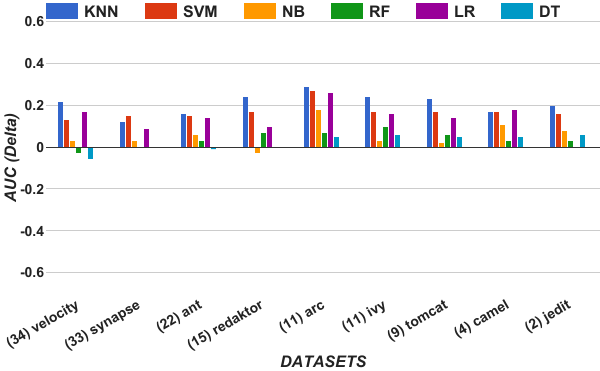
\includegraphics[width=.95\linewidth]{./fig/AUC_untuned.png}
        
  {\bf Figure~\ref{fig:untuned}a:} AUC (pf, recall)
        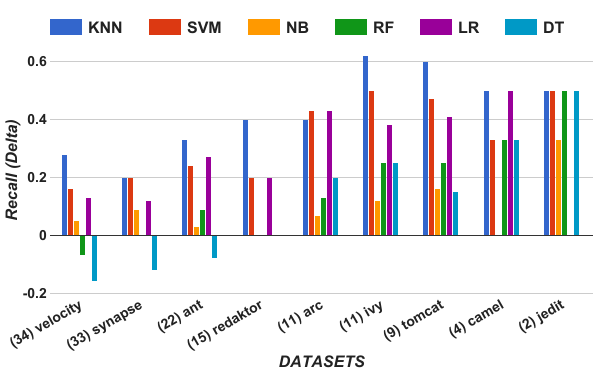
\includegraphics[width=.95\linewidth]{./fig/Recall_untuned.png}
  {\bf Figure~\ref{fig:untuned}c:} Recall
    \end{minipage}%
\begin{minipage}{.5\linewidth}
        \centering
        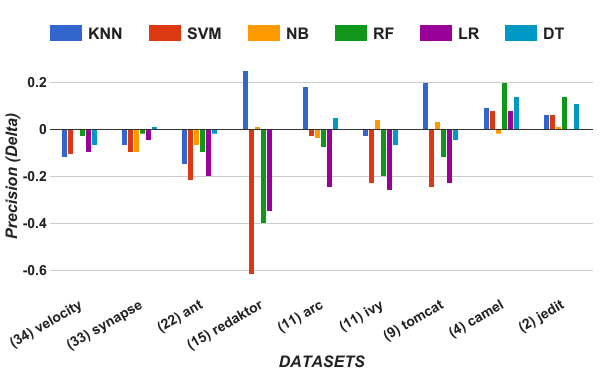
\includegraphics[width=.95\linewidth]{./fig/prec_untuned.png}
  {\bf Figure~\ref{fig:untuned}b:} Precision
        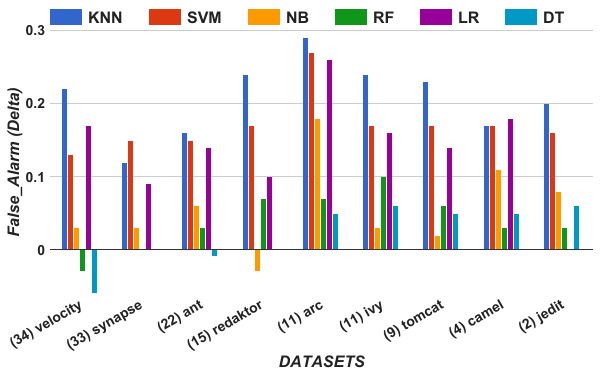
\includegraphics[width=.95\linewidth]{./fig/pf_untuned.png}
  {\bf Figure~\ref{fig:untuned}d:} False Alarm
    \end{minipage}%
    \caption{SMOTE1 improvement over No SMOTE. Legends represent the classifiers mentioned in \tion{classes}}
    \label{fig:untuned}
\end{figure*}

\begin{figure*}[!t]
\begin{minipage}{.5\linewidth}
\centering
        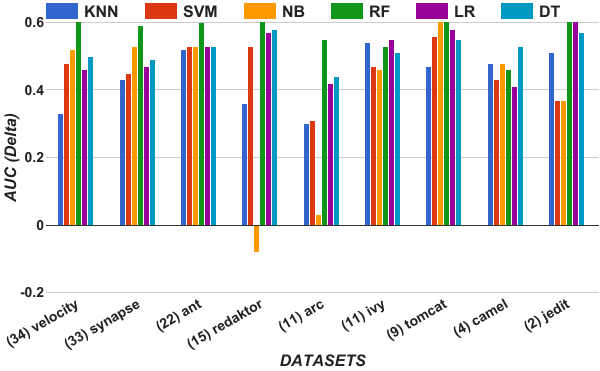
\includegraphics[width=.95\linewidth]{./fig/AUC_tuned.png}
        
  {\bf Figure~\ref{fig:tuned}a:} AUC (pf, recall)
        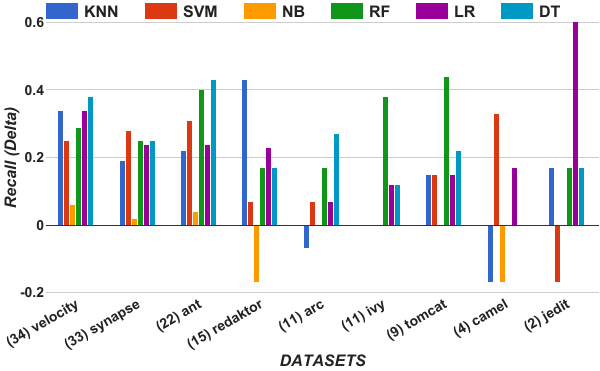
\includegraphics[width=.95\linewidth]{./fig/Recall_tuned.png}
  {\bf Figure~\ref{fig:tuned}c:} Recall
    \end{minipage}%
\begin{minipage}{.5\linewidth}
        \centering
        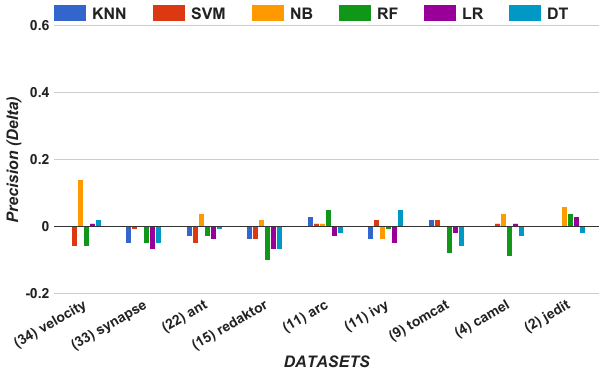
\includegraphics[width=.95\linewidth]{./fig/prec_tuned.png}
  {\bf Figure~\ref{fig:tuned}b:} Precision
        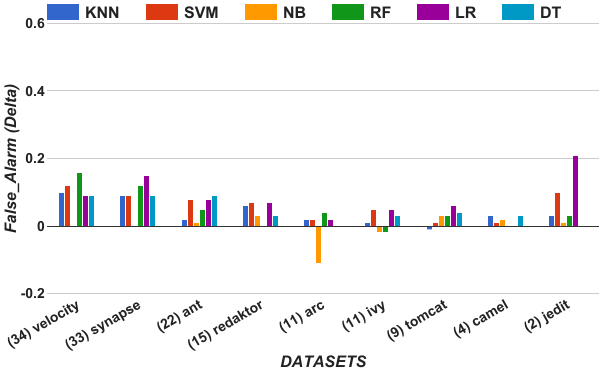
\includegraphics[width=.95\linewidth]{./fig/pf_tuned.png}
  {\bf Figure~\ref{fig:tuned}d:} False Alarm
    \end{minipage}%
    \caption{SMOTE2 improvement over SMOTE1. Legends represent the classifiers mentioned in \tion{classes}.}
    \label{fig:tuned}
\end{figure*}

\section{Results}
\label{sect:results}

\subsection{\textbf{RQ1: Is standard ``off-the-shelf'' SMOTE1 preprocessing method important for defect prediction?}}
Figure~\ref{fig:untuned} represents the improvement of SMOTE1 (median value) against the No SMOTE (median value) results and Figure~\ref{fig:tuned} represents the improvement of SMOTE2 (median value) against SMOTE1 (median value) results. Each figure contains subfigures for all our 4 evaluation measures (mentioned in \tion{measure}) compared with 6 learners (mentioned in \tion{classes}). 



For subfigures (AUC, Recall and Precision) in each Figure~\ref{fig:untuned} and \ref{fig:tuned}:
\bi
\item 
{\em Larger} y-values
are {\em better} 
\item
If the y-value goes {\em negative}, then the corresponding learner performs {\em worse}. 
\ei
For the false alarms, the
plots must be interpreted differently:
\bi
\item
{\em Larger} y-values are {\em worse};
\item
If the y-value goes {\em positive} then
the corresponding leaner
performs {\em worse}.
\ei
Note that, using SMOTE1 on KNN, SVM,
LR (linear regression) often
leads to much larger false alarm increases.
On the other hand,   NB
and RF have much smaller
increase in false alarm.

In these figures, the
X-axis shows all 9 data sets in the decreasing percentage of defective classes from left to right. The corresponding percentage of minority class (in this case, defective class) is written beside each data set. Note that:
\bi
\item
According to the proponents
of SMOTE, SMOTE's improvements should
{\em increase} as we move left to right
across those plots.
\item
No such trend exists in our results for
AUC, precision or false alarms.
\item
For recall, looking left-to-right across
Figure~\ref{fig:untuned}c, we can see
large positive increases on the
right-hand-side than the left.
\ei
% Based on these results,  we can best recommend SMOTE1 when:
% \bi
% \item Trying to improve recall
% for imbalanaced data sets;
% \item
% Using NB or Random Forests.
% \ei

% For SMOTE2 improvement over SMOTE1 (figure~\ref{fig:tuned}), AUC values are shown in subfigure~\ref{fig:tuned}a. Redaktor data set is selected from X-axis, and yellow bar represents NB which corresponds to about $-0.08$ AUC value. This denotes that NB performed worse by tuning the parameters of SMOTE1. The original parameter settings of SMOTE1 worked the best. On the other hand for the same data set, KNN (which is represented in dark blue bar) shows the AUC value of $0.35$. This shows KNN outperformed the ``off-the-shelf'' SMOTE1 when tuned using DE.



% By looking at the results of AUC from figure~\ref{fig:untuned}a, only 4 bars are negative, and rest all the remaining 50 bars (in total 9 data sets with 6 learners in each) have  positive effect by using SMOTE1 as a preprocessing method. We are seeing a maximum improvement of about 30\%. These improvements are quite modest as to ignore the importance of SMOTE.

% Results for precision (in figure~\ref{fig:untuned}b), are not much interesting, but the decrease in precision value is not that arduous except for the redaktor data set. Though we will not recommend using SMOTE whenever we want higher precision value. Since precision is decreased using SMOTE, it was expected to have increased false alarm \cite{menzies2007problems} and the same is observed from figure~\ref{fig:untuned}d. There is an increase in error among false positives but the increase is very minimal.

% As for recall (figure~\ref{fig:untuned}c), only 4 bars are negative, and rest all the remaining 50 bars (in total 9 data sets with 6 learners in each) have positive effect by using SMOTE1. We are seeing a maximum improvement of about 60\%. These improvements are quite steep as to ignore the importance of SMOTE at any point for any learner. It is also observed that performance keeps increasing as target class becomes more minor and minor. This is what was expected after applying SMOTE to imbalance data sets.

\noindent
Summarizing the above:
\begin{lesson1}
We can recommend SMOTE1 for improving recall, and modest improvements in AUC. But  SMOTE1 adversely effect
precision.
\end{lesson1}

\subsection{\textbf{RQ2: Can tuning SMOTE1 achieve better results?}}

Figure~\ref{fig:tuned} shows the results
after applying SMOTE2. All these
plots show the {\em delta} between
the SMOTE1 results and those of SMOTE2.
As before, {\em positive}  values
are better for AUC, recall and precision
wile {\em negative} values are better for false alarms.

The benefit of SMOTE2's tunings are clearly evident in the AUC results of  Figure~\ref{fig:tuned}a:
all learners show large performance improvements. 
Better yet,  as
shown in
Figure~\ref{fig:tuned}b, and Figure~\ref{fig:tuned}d, SMOTE2 does
not adversely effect false alarm and precision.

SMOTE2's benefits for recall are not very
strong (and seem to be strongest for the more balanced data sets on the left-hand-side of Figure~\ref{fig:tuned}c)
but are rarely negative.




% results are dramat
% Now when we look at the results of AUC from figure~\ref{fig:tuned}a, only 1 bar is negative, and rest all the remaining 53 bars (in total 9 data sets with 6 learners in each) have  positive effect after when we tune the parameters of SMOTE1. We are seeing a maximum improvement of about 70\% and on an average 50\% for each learner in all data sets. These improvements are quite steep in nature and just to remind you that these results are improvement over SMOTE1. If we combine the results, then we can surely say to tune the parameters of SMOTE1 and train using any learner, we will get atleast 100\% improvement in most cases.

% We are seeing the similar trend of results for precision (in figure~\ref{fig:tuned}b), just like in Figure~\ref{fig:untuned}b, that even after tuning for precision, we are not seeing much improvement. Though we definitely improved precision slightly than SMOTE1 but the increment is not that large to recommend SMOTE2 or SMOTE1. And even after trying to minimise the false alarm (figure~\ref{fig:tuned}d) value, DE could not find a good parameter setting.

% As for recall (figure~\ref{fig:untuned}c), only 5 bars are negative, and rest all the remaining 49 bars (in total 9 data sets with 6 learners in each) have either positive effect or no effect after tuning. We are seeing a maximum improvement of about 65\% but the average improvement is close to 15\% for each classifiers in all data sets. But these improvements combined with SMOTE1 suggest that we should always tune SMOTE1 whenever the goal is to achieve higher recall.
In summary:

\begin{lesson1}
    For defect data, SMOTE2  
 offers   some  improvements over SMOTE1 for recall
 and dramatic improvements for AUC (pf, recall) without damaging precision or false
 alarm.
\end{lesson1}

Overall, in  Figure~\ref{fig:tuned},
there are very few negative results
(except in precision, where the negatives
are very small). That is, there
seems little to be lost using SMOTE2
but much to gain (e.g. the large AUC improvements).
Based on these results, we strongly
recommend SMOTE2 for handling unbalanced
data sets.

\begin{figure*}[!t]
    \centering
    \begin{minipage}{.33\textwidth}
        \captionsetup{justification=centering,singlelinecheck=off}
        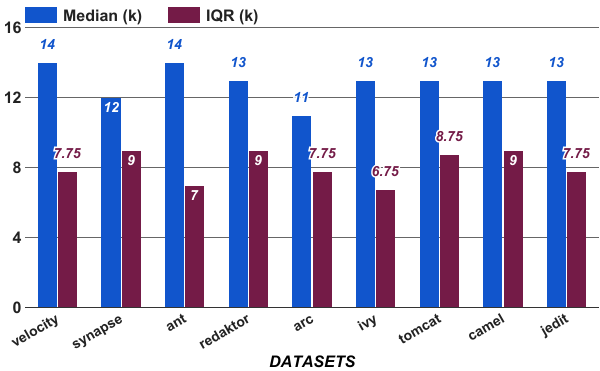
\includegraphics[width=.95\linewidth]{./fig/k.png}
        \caption{Data sets vs Parameter ($k$) variation}
        \label{RQ3:k}
    \end{minipage}%
    \begin{minipage}{.33\textwidth}
        \captionsetup{labelsep=space,justification=centering,singlelinecheck=off}
        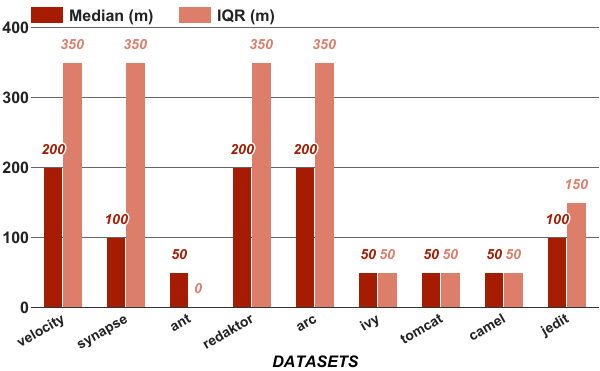
\includegraphics[width=.95\linewidth]{./fig/m.png}
        \caption{Data sets vs Parameter ($m$) variation}
        \label{RQ3:a}
    \end{minipage}
    \begin{minipage}{.33\textwidth}
        \captionsetup{labelsep=space,justification=centering,singlelinecheck=off}
        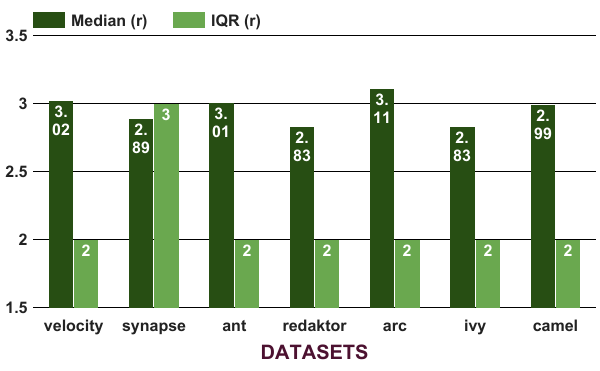
\includegraphics[width=.95\linewidth]{./fig/r.png}
        \caption{Data sets vs Parameter ($r$) variation}
        \label{RQ3:b}
    \end{minipage}
\end{figure*}

\subsection{\textbf{RQ3: Do different data sets
      need different configurations with SMOTE2?}}

Figures \ref{RQ3:k}, \ref{RQ3:a}, and \ref{RQ3:b} show the results of tuning for each data set when recall is considered as evaluation goal. These parameter settings are found by each learner for that data set.
On display in each set of vertical bars are
the median values generated across 15 evaluations.
Also, shown are
the inter-quartile range (IQR) of those tunings (the IQR is the 75th-25th percentile values and is a non-parametric measure of variation
around the median value). Note that in Figure \ref{RQ3:a}, IQR=0 for  ant data set where tuning
          always converged on the same final value.

  These figures
show how tuning selects the different ranges  of
parameters.
Some of the above numbers are far from the standard values; e.g. Chawla et al.~\cite{chawla2002smote} recommend using $k=5$ neighbors yet in our data sets, best results were seen using $k \approx 13$. On other hand it was suggested to use $m=900$ by ~\cite{pears2014synthetic}.
Clearly,
best results from tuning
vary with each data set.

Clearly:
\begin{lesson1}
    DE finds different ``best'' parameter settings for SMOTE2 for different data sets.
\end{lesson1}
 That is,  reusing tunings  suggested  by  any other  previous study  for any data set is \underline{{\em not}} recommended. Instead,  it is better to
      use  automatic  tuning  methods  to find the best tuning parameters for the current data set.
      

\begin{figure}[!t]
  \captionsetup{justification=centering}
  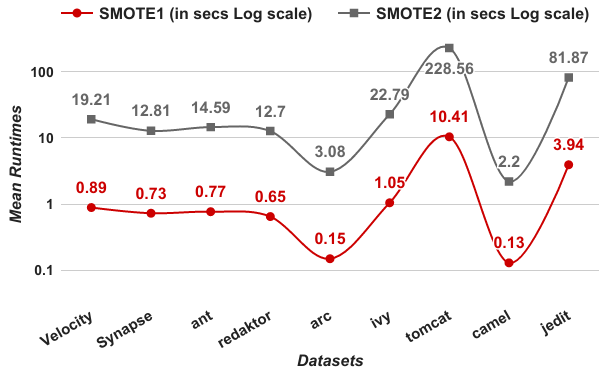
\includegraphics[width=\linewidth]{./fig/runtimes.png}
  \caption{Data sets vs Runtimes}
  \label{runtime}
\end{figure} 

\subsection{\textbf{RQ4: Is tuning impractically slow?}}

Search-based SE methods can be very slow. Wang et al.~\cite{wang2013searching} once needed 15
years of CPU time to find and verify the tunings required for software
clone detectors. Sayyad et al.~\cite{sayyad2013scalable} routinely used
$10^6$ evaluations (or more) of their models in order to extract
products from highly constrained product
lines. Hence, before recommending any
search-based method, it is wise to consider the runtime cost of that
recommendation.

To understand our timing results, recall that SMOTE2 uses
Algorithm~1. Based on the psuedocode
shown above, our pre-experimental expectation is that
tuning will be three to fives times slower than not tuning.  
Figure~\ref{runtime} checks if that theoretical
holds true in practice. Shown in circle and square markers are the
  runtimes required to run SMOTE1 and SMOTE2 respectively.  The
  longer runtimes (in square) include the times required for DE to find
  the tunings. Overall, tuning slows down the training by a factor of up to
  five (which is very close to our theoretical prediction).

\begin{lesson1}
    Tuning with DE makes training four to five times slower, but the improvements which we get for AUC and recall is quite advantageous.
\end{lesson1}


\begin{figure}[!htbp]
\begin{minipage}{\linewidth}
\centering
        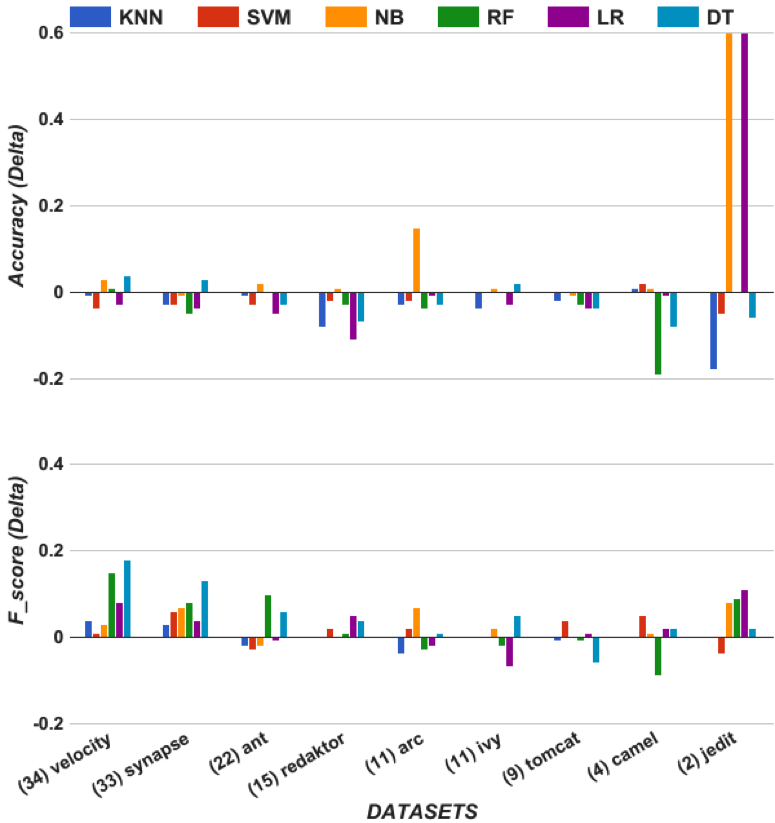
\includegraphics[width=.95\linewidth]{./fig/acc_f_tuned.png}
    \end{minipage}%
    \caption{SMOTE2 improvement over SMOTE1. Legends represent the classifiers mentioned in \tion{classes}}
    \label{fig:threats}
\end{figure}

\section{Threats to Validity}
\label{sect:validity}

As with any empirical study, biases can affect the final
results. Therefore, any conclusions made from this work must be considered with the following issues in mind:

\textbf{\textit{Sampling bias}} threatens any classification experiment; i.e., what matters there may not be true here. For example, the data sets used here comes from the PROMISE~\cite{promiserepo} repository and were supplied by one individual. But these data sets have used in various case studies by various researchers~\cite{he2012investigation,peters2013better,peters2013balancing,turhan2013empirical} making our results more conclusive.
Though we have used 9 open-source data sets for Software Defect prediction (Table~\ref{tb:dataset}) which are mostly from Apache, and some are proprietary projects, there could be other data sets for which our results could be wrong.

\textbf{\textit{Learner bias}}: For building the defect predictors in this
study, we selected each learner with default parameters like k=8 in $k$-NN, entropy as split criteria in RF, and DT. The above predefined parameters have been used in the conclusions made by other studies~\cite{ghotra2015revisiting,tantithamthavorn2016automated}. But classification is a large and active field and any single study can only use a small subset of the known classification algorithms.

\textbf{\textit{Evaluation bias}}: Most highly cited papers~\cite{ghotra2015revisiting,tantithamthavorn2016automated} have only concluded using $AUC\ (pf, recall)$ whereas we went ahead and are reporting 3 other measures. There are other measures used in software engineering which includes Accuracy, Fscore. But we still performed SMOTE2 on Fscore and Accuracy and did not find any improvement (Figure~\ref{fig:threats}). Anyway, accuracy is not the best measure to report for defect prediction as we do not want any true negative numbers included. Fscore is the harmonic mean of precision and recall and if you recall our SMOTE2 results, we see  increment in recall as well as  decrement in precision making Fscore negligible.

\textbf{\textit{Order bias}}: With each data set how data samples are distributed in training and testing set is completely random. Though there could be times when all good samples are binned into training and testing set. To mitigate this order bias, we run
the experiment 25 times by randomly changing the order of the data samples each time.

\section{Conclusion}
\label{sect:conclusion}

Based on the above, we offer a specific and general conclusion. Most specifically, we recommend.
\bi
 %\item Previous studies~\cite{ghotra2015revisiting,tantithamthavorn2016automated} have mostly reported on only 1 evaluation goal, but we reported on many.
 \item Any study~\cite{ghotra2015revisiting} that has reported AUC without studying the effects of class imbalance needs to be analyzed again by applying SMOTE. We say this since SMOTE2 showed big improvements in AUC.
% \item Whenever we want to maximise a certain evaluation goal, specifically AUC and recall, then it is recommended to tune the parameters of SMOTE1.
 \item Unlike the advise of Chawal et al.~\cite{chawla2002smote} of using $k=5$ for SMOTE, we should have automatic methods like DE to tune the parameters of SMOTE and find the best parameter settings.
 \item Do not use someone else's pre-tuned SMOTE, since, as shown here, the best tunings vary from data set to data set.
\ei
Based on our runtime results, we can say that list last
recommendation (to tune before applying analytics) is not  a particular
onerous demand. The additional cost of tuning
is relatively minor while the benefits of the SMTOE2 tunings
are very large (see the   AUC and recall results shown above),

% In the future, we plan to work on other similar issues like:
% \bi
%  \item Tuning SMOTE and learners at the same time and comparing against the results of No SMOTE, SMOTE1, and SMOTE2.
%  \item Predicting the quantities of defects which is regression based model rather having a binary based classification model with tuning.
% \ei
\newpage

\balance

\bibliographystyle{ACM-Reference-Format}
\medskip
\bibliography{main}

\end{document}